% Created by tikzDevice version 0.12.6 on 2026-08-08 12:10:47
% !TEX encoding = UTF-8 Unicode
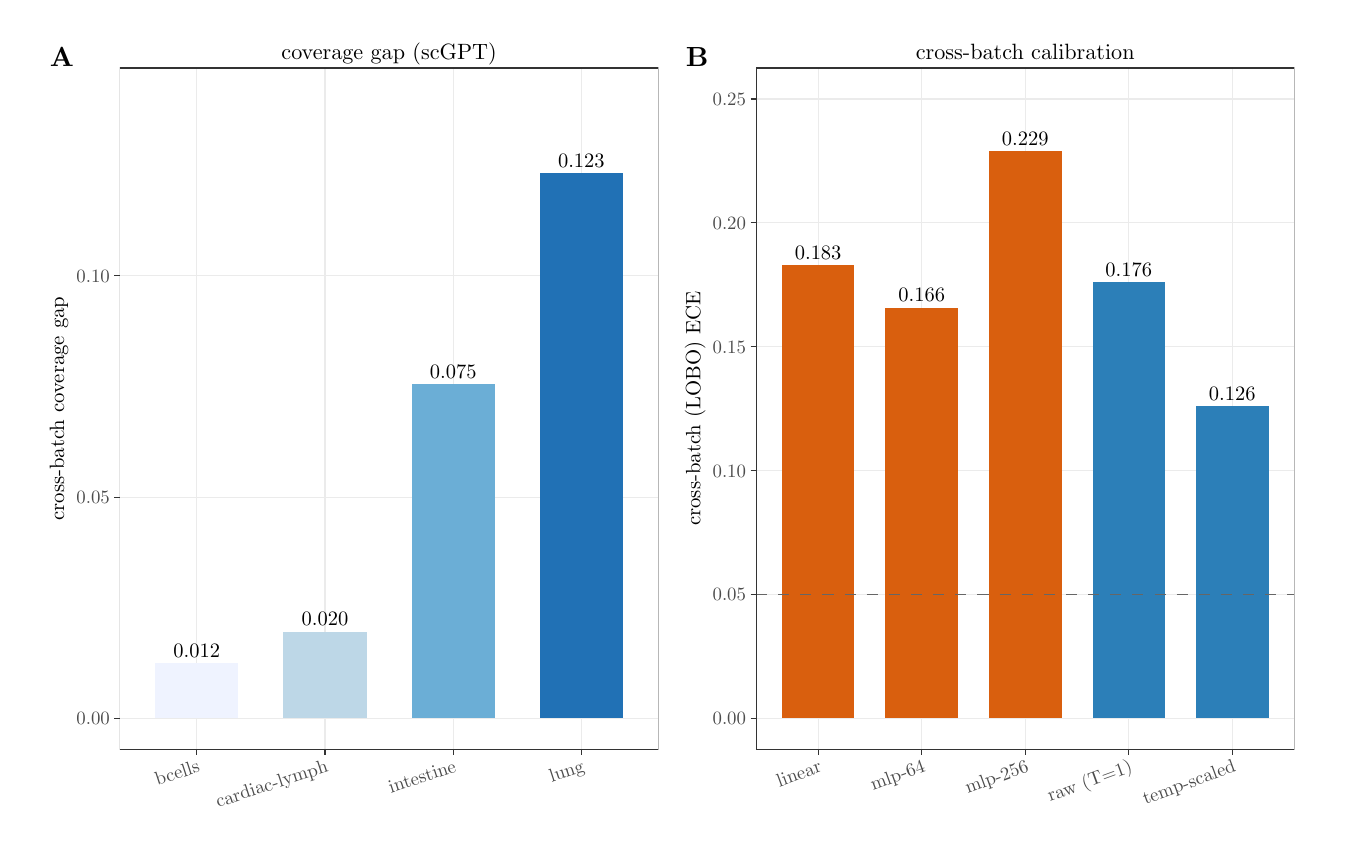
\begin{tikzpicture}[x=1pt,y=1pt]
\definecolor{fillColor}{RGB}{255,255,255}
\path[use as bounding box,fill=fillColor,fill opacity=0.00] (0,0) rectangle (469.75,289.08);
\begin{scope}
\path[clip] (  0.00,  0.00) rectangle (469.75,289.08);
\definecolor{drawColor}{RGB}{255,255,255}
\definecolor{fillColor}{RGB}{255,255,255}

\path[draw=drawColor,line width= 0.4pt,line join=round,line cap=round,fill=fillColor] ( -0.00,  0.00) rectangle (469.76,289.08);
\end{scope}
\begin{scope}
\path[clip] (  4.00,  3.00) rectangle (233.88,286.08);
\definecolor{drawColor}{RGB}{255,255,255}
\definecolor{fillColor}{RGB}{255,255,255}

\path[draw=drawColor,line width= 0.4pt,line join=round,line cap=round,fill=fillColor] (  4.00,  3.00) rectangle (233.88,286.08);
\end{scope}
\begin{scope}
\path[clip] (233.88,  3.00) rectangle (463.76,286.08);
\definecolor{drawColor}{RGB}{255,255,255}
\definecolor{fillColor}{RGB}{255,255,255}

\path[draw=drawColor,line width= 0.4pt,line join=round,line cap=round,fill=fillColor] (233.88,  3.00) rectangle (463.75,286.08);
\end{scope}
\begin{scope}
\path[clip] ( 33.31, 28.33) rectangle (227.88,274.52);
\definecolor{fillColor}{RGB}{255,255,255}

\path[fill=fillColor] ( 33.31, 28.33) rectangle (227.88,274.52);
\definecolor{drawColor}{gray}{0.92}

\path[draw=drawColor,line width= 0.4pt,line join=round] ( 33.31, 39.52) --
	(227.88, 39.52);

\path[draw=drawColor,line width= 0.4pt,line join=round] ( 33.31,119.45) --
	(227.88,119.45);

\path[draw=drawColor,line width= 0.4pt,line join=round] ( 33.31,199.38) --
	(227.88,199.38);

\path[draw=drawColor,line width= 0.4pt,line join=round] ( 61.10, 28.33) --
	( 61.10,274.52);

\path[draw=drawColor,line width= 0.4pt,line join=round] (107.43, 28.33) --
	(107.43,274.52);

\path[draw=drawColor,line width= 0.4pt,line join=round] (153.76, 28.33) --
	(153.76,274.52);

\path[draw=drawColor,line width= 0.4pt,line join=round] (200.08, 28.33) --
	(200.08,274.52);
\definecolor{fillColor}{RGB}{33,113,181}

\path[fill=fillColor] (185.03, 39.52) rectangle (215.14,236.63);
\definecolor{fillColor}{RGB}{239,243,255}

\path[fill=fillColor] ( 46.05, 39.52) rectangle ( 76.16, 59.34);
\definecolor{fillColor}{RGB}{189,215,231}

\path[fill=fillColor] ( 92.37, 39.52) rectangle (122.49, 70.85);
\definecolor{fillColor}{RGB}{107,174,214}

\path[fill=fillColor] (138.70, 39.52) rectangle (168.81,160.21);
\definecolor{drawColor}{RGB}{0,0,0}

\node[text=drawColor,anchor=base,inner sep=0pt, outer sep=0pt, scale=  0.74] at (200.08,238.67) {0.123};

\node[text=drawColor,anchor=base,inner sep=0pt, outer sep=0pt, scale=  0.74] at ( 61.10, 61.38) {0.012};

\node[text=drawColor,anchor=base,inner sep=0pt, outer sep=0pt, scale=  0.74] at (107.43, 72.89) {0.020};

\node[text=drawColor,anchor=base,inner sep=0pt, outer sep=0pt, scale=  0.74] at (153.76,162.25) {0.075};
\definecolor{drawColor}{gray}{0.20}

\path[draw=drawColor,line width= 0.4pt,line join=round,line cap=round] ( 33.31, 28.33) rectangle (227.88,274.52);
\end{scope}
\begin{scope}
\path[clip] (  0.00,  0.00) rectangle (469.75,289.08);
\definecolor{drawColor}{gray}{0.30}

\node[text=drawColor,anchor=base east,inner sep=0pt, outer sep=0pt, scale=  0.68] at ( 29.71, 37.18) {0.00};

\node[text=drawColor,anchor=base east,inner sep=0pt, outer sep=0pt, scale=  0.68] at ( 29.71,117.11) {0.05};

\node[text=drawColor,anchor=base east,inner sep=0pt, outer sep=0pt, scale=  0.68] at ( 29.71,197.04) {0.10};
\end{scope}
\begin{scope}
\path[clip] (  0.00,  0.00) rectangle (469.75,289.08);
\definecolor{drawColor}{gray}{0.20}

\path[draw=drawColor,line width= 0.4pt,line join=round] ( 31.31, 39.52) --
	( 33.31, 39.52);

\path[draw=drawColor,line width= 0.4pt,line join=round] ( 31.31,119.45) --
	( 33.31,119.45);

\path[draw=drawColor,line width= 0.4pt,line join=round] ( 31.31,199.38) --
	( 33.31,199.38);
\end{scope}
\begin{scope}
\path[clip] (  0.00,  0.00) rectangle (469.75,289.08);
\definecolor{drawColor}{gray}{0.20}

\path[draw=drawColor,line width= 0.4pt,line join=round] ( 61.10, 26.33) --
	( 61.10, 28.33);

\path[draw=drawColor,line width= 0.4pt,line join=round] (107.43, 26.33) --
	(107.43, 28.33);

\path[draw=drawColor,line width= 0.4pt,line join=round] (153.76, 26.33) --
	(153.76, 28.33);

\path[draw=drawColor,line width= 0.4pt,line join=round] (200.08, 26.33) --
	(200.08, 28.33);
\end{scope}
\begin{scope}
\path[clip] (  0.00,  0.00) rectangle (469.75,289.08);
\definecolor{drawColor}{gray}{0.30}

\node[text=drawColor,rotate= 18.00,anchor=base east,inner sep=0pt, outer sep=0pt, scale=  0.68] at ( 62.55, 20.28) {bcells};

\node[text=drawColor,rotate= 18.00,anchor=base east,inner sep=0pt, outer sep=0pt, scale=  0.68] at (108.88, 20.28) {cardiac-lymph};

\node[text=drawColor,rotate= 18.00,anchor=base east,inner sep=0pt, outer sep=0pt, scale=  0.68] at (155.20, 20.28) {intestine};

\node[text=drawColor,rotate= 18.00,anchor=base east,inner sep=0pt, outer sep=0pt, scale=  0.68] at (201.53, 20.28) {lung};
\end{scope}
\begin{scope}
\path[clip] (  0.00,  0.00) rectangle (469.75,289.08);
\definecolor{drawColor}{RGB}{0,0,0}

\node[text=drawColor,rotate= 90.00,anchor=base,inner sep=0pt, outer sep=0pt, scale=  0.75] at ( 13.17,151.42) {cross-batch coverage gap};
\end{scope}
\begin{scope}
\path[clip] (  0.00,  0.00) rectangle (469.75,289.08);
\definecolor{drawColor}{RGB}{0,0,0}

\node[text=drawColor,anchor=base,inner sep=0pt, outer sep=0pt, scale=  0.80] at (130.59,277.57) {coverage gap (scGPT)};
\end{scope}
\begin{scope}
\path[clip] (  0.00,  0.00) rectangle (469.75,289.08);
\definecolor{drawColor}{RGB}{0,0,0}

\node[text=drawColor,anchor=base,inner sep=0pt, outer sep=0pt, scale=  1.00] at ( 12.35,275.21) {\bfseries A};
\end{scope}
\begin{scope}
\path[clip] (263.19, 28.33) rectangle (457.75,274.52);
\definecolor{fillColor}{RGB}{255,255,255}

\path[fill=fillColor] (263.19, 28.33) rectangle (457.75,274.52);
\definecolor{drawColor}{gray}{0.92}

\path[draw=drawColor,line width= 0.4pt,line join=round] (263.19, 39.52) --
	(457.75, 39.52);

\path[draw=drawColor,line width= 0.4pt,line join=round] (263.19, 84.28) --
	(457.75, 84.28);

\path[draw=drawColor,line width= 0.4pt,line join=round] (263.19,129.04) --
	(457.75,129.04);

\path[draw=drawColor,line width= 0.4pt,line join=round] (263.19,173.80) --
	(457.75,173.80);

\path[draw=drawColor,line width= 0.4pt,line join=round] (263.19,218.56) --
	(457.75,218.56);

\path[draw=drawColor,line width= 0.4pt,line join=round] (263.19,263.32) --
	(457.75,263.32);

\path[draw=drawColor,line width= 0.4pt,line join=round] (285.64, 28.33) --
	(285.64,274.52);

\path[draw=drawColor,line width= 0.4pt,line join=round] (323.05, 28.33) --
	(323.05,274.52);

\path[draw=drawColor,line width= 0.4pt,line join=round] (360.47, 28.33) --
	(360.47,274.52);

\path[draw=drawColor,line width= 0.4pt,line join=round] (397.89, 28.33) --
	(397.89,274.52);

\path[draw=drawColor,line width= 0.4pt,line join=round] (435.30, 28.33) --
	(435.30,274.52);
\definecolor{fillColor}{RGB}{217,95,14}

\path[fill=fillColor] (272.54, 39.52) rectangle (298.73,203.17);

\path[fill=fillColor] (309.96, 39.52) rectangle (336.15,187.95);

\path[fill=fillColor] (347.37, 39.52) rectangle (373.57,244.61);
\definecolor{fillColor}{RGB}{44,127,184}

\path[fill=fillColor] (384.79, 39.52) rectangle (410.98,197.26);

\path[fill=fillColor] (422.21, 39.52) rectangle (448.40,152.50);
\definecolor{drawColor}{RGB}{0,0,0}

\node[text=drawColor,anchor=base,inner sep=0pt, outer sep=0pt, scale=  0.74] at (285.64,205.20) {0.183};

\node[text=drawColor,anchor=base,inner sep=0pt, outer sep=0pt, scale=  0.74] at (323.05,189.99) {0.166};

\node[text=drawColor,anchor=base,inner sep=0pt, outer sep=0pt, scale=  0.74] at (360.47,246.65) {0.229};

\node[text=drawColor,anchor=base,inner sep=0pt, outer sep=0pt, scale=  0.74] at (397.89,199.30) {0.176};

\node[text=drawColor,anchor=base,inner sep=0pt, outer sep=0pt, scale=  0.74] at (435.30,154.53) {0.126};
\definecolor{drawColor}{gray}{0.40}

\path[draw=drawColor,line width= 0.4pt,dash pattern=on 4pt off 4pt ,line join=round] (263.19, 84.28) -- (457.75, 84.28);
\definecolor{drawColor}{gray}{0.20}

\path[draw=drawColor,line width= 0.4pt,line join=round,line cap=round] (263.19, 28.33) rectangle (457.75,274.52);
\end{scope}
\begin{scope}
\path[clip] (  0.00,  0.00) rectangle (469.75,289.08);
\definecolor{drawColor}{gray}{0.30}

\node[text=drawColor,anchor=base east,inner sep=0pt, outer sep=0pt, scale=  0.68] at (259.59, 37.18) {0.00};

\node[text=drawColor,anchor=base east,inner sep=0pt, outer sep=0pt, scale=  0.68] at (259.59, 81.94) {0.05};

\node[text=drawColor,anchor=base east,inner sep=0pt, outer sep=0pt, scale=  0.68] at (259.59,126.70) {0.10};

\node[text=drawColor,anchor=base east,inner sep=0pt, outer sep=0pt, scale=  0.68] at (259.59,171.46) {0.15};

\node[text=drawColor,anchor=base east,inner sep=0pt, outer sep=0pt, scale=  0.68] at (259.59,216.22) {0.20};

\node[text=drawColor,anchor=base east,inner sep=0pt, outer sep=0pt, scale=  0.68] at (259.59,260.98) {0.25};
\end{scope}
\begin{scope}
\path[clip] (  0.00,  0.00) rectangle (469.75,289.08);
\definecolor{drawColor}{gray}{0.20}

\path[draw=drawColor,line width= 0.4pt,line join=round] (261.19, 39.52) --
	(263.19, 39.52);

\path[draw=drawColor,line width= 0.4pt,line join=round] (261.19, 84.28) --
	(263.19, 84.28);

\path[draw=drawColor,line width= 0.4pt,line join=round] (261.19,129.04) --
	(263.19,129.04);

\path[draw=drawColor,line width= 0.4pt,line join=round] (261.19,173.80) --
	(263.19,173.80);

\path[draw=drawColor,line width= 0.4pt,line join=round] (261.19,218.56) --
	(263.19,218.56);

\path[draw=drawColor,line width= 0.4pt,line join=round] (261.19,263.32) --
	(263.19,263.32);
\end{scope}
\begin{scope}
\path[clip] (  0.00,  0.00) rectangle (469.75,289.08);
\definecolor{drawColor}{gray}{0.20}

\path[draw=drawColor,line width= 0.4pt,line join=round] (285.64, 26.33) --
	(285.64, 28.33);

\path[draw=drawColor,line width= 0.4pt,line join=round] (323.05, 26.33) --
	(323.05, 28.33);

\path[draw=drawColor,line width= 0.4pt,line join=round] (360.47, 26.33) --
	(360.47, 28.33);

\path[draw=drawColor,line width= 0.4pt,line join=round] (397.89, 26.33) --
	(397.89, 28.33);

\path[draw=drawColor,line width= 0.4pt,line join=round] (435.30, 26.33) --
	(435.30, 28.33);
\end{scope}
\begin{scope}
\path[clip] (  0.00,  0.00) rectangle (469.75,289.08);
\definecolor{drawColor}{gray}{0.30}

\node[text=drawColor,rotate= 20.00,anchor=base east,inner sep=0pt, outer sep=0pt, scale=  0.68] at (287.24, 20.33) {linear};

\node[text=drawColor,rotate= 20.00,anchor=base east,inner sep=0pt, outer sep=0pt, scale=  0.68] at (324.66, 20.33) {mlp-64};

\node[text=drawColor,rotate= 20.00,anchor=base east,inner sep=0pt, outer sep=0pt, scale=  0.68] at (362.07, 20.33) {mlp-256};

\node[text=drawColor,rotate= 20.00,anchor=base east,inner sep=0pt, outer sep=0pt, scale=  0.68] at (399.49, 20.33) {raw (T=1)};

\node[text=drawColor,rotate= 20.00,anchor=base east,inner sep=0pt, outer sep=0pt, scale=  0.68] at (436.91, 20.33) {temp-scaled};
\end{scope}
\begin{scope}
\path[clip] (  0.00,  0.00) rectangle (469.75,289.08);
\definecolor{drawColor}{RGB}{0,0,0}

\node[text=drawColor,rotate= 90.00,anchor=base,inner sep=0pt, outer sep=0pt, scale=  0.75] at (243.04,151.42) {cross-batch (LOBO) ECE};
\end{scope}
\begin{scope}
\path[clip] (  0.00,  0.00) rectangle (469.75,289.08);
\definecolor{drawColor}{RGB}{0,0,0}

\node[text=drawColor,anchor=base,inner sep=0pt, outer sep=0pt, scale=  0.80] at (360.47,277.57) {cross-batch calibration};
\end{scope}
\begin{scope}
\path[clip] (  0.00,  0.00) rectangle (469.75,289.08);
\definecolor{drawColor}{RGB}{0,0,0}

\node[text=drawColor,anchor=base,inner sep=0pt, outer sep=0pt, scale=  1.00] at (241.97,275.21) {\bfseries B};
\end{scope}
\end{tikzpicture}
